% INTRODUÇÃO-------------------------------------------------------------------

\chapter{Introdução}
\label{chap:introducao}

% Sugestão da professora Leyza
% 1 Parágrafo de contextualização
% 2 Parágrafos com o problema (justificativa)
% 1 parágrafo mencionando estado da arte
% 2/3 parágrafos com a solução (método proposto e resultados parciais)
% 1 parágrafo com organização do trabalho

Esteganografia pode ser definida como a comunicação de uma mensagem secreta escondida em uma mídia, a qual pode ser qualquer objeto cuja estrutura permita que pequenas alterações sejam realizadas para codificar a mensagem dificultando sua detecção~\cite{fridrich2009steganography}.

Suponha que duas partes, \textit{Alice} e \textit{Bob}, queiram trocar mensagens através do uso de esteganografia, i.e., se comunicar secretamente de tal forma que \textit{Eve} não detecte que tal comunicação está em curso. São reconhecidas cinco etapas fundamentais para uma comunicação secreta utilizando esteganografia~\cite{fridrich2009steganography}:

\begin{enumerate}
	\item \textit{Alice} e \textit{Bob} escolhem os objetos que irão ocultar a mensagem. Tais objetos devem ser comuns no canal que \textit{Eve} está monitorando, de tal forma que eles não sejam identificados como estranhos e, consequentemente, relacionados facilmente a  uma mensagem secreta.
	\item \textit{Alice} e \textit{Bob} precisam desenvolver ou escolher implementações de algoritmos para embutir e extrair os dados secretos dos objetos.
	\item Opcionalmente, para aumentar a segurança da comunicação, \textit{Alice} e \textit{Bob} podem estipular uma senha previamente, sendo que somente quem a possui consegue extrair a mensagem secreta do objeto.
	\item \textit{Alice} deve embutir a mensagem nos objetos escolhidos.
	\item \textit{Alice} envia os objetos com a mensagem embutida através do canal de comunicação potencialmente não confiável, para finalmente, \textit{Bob} extrair a mensagem.
\end{enumerate}

Para conseguir detectar que mensagens secretas estão sendo trocadas, \textit{Eve} deverá utilizar técnicas de esteganálise nos objetos aparentemente inofensivos. Esteganálise é o estudo de métodos para a extração de atributos da esteganografia dada uma mídia suspeita. Esses atributos podem ser, por exemplo, se existe ou não uma mensagem escondida, o tamanho da mensagem, possíveis informações sobre a chave, localização da mensagem na mídia, dedução da mensagem, entre outros.%~\cite{fridrich2009steganography}.

Na década passada, ocorreu um interesse crescente na área de esteganografia e esteganálise devido à disseminação da internet e de mídias digitais, as quais criam um ambiente favorável para a comunicação oculta (dado que são comumente representadas por uma grande quantidade de amostras e ruídos, os quais podem ser modificados imperceptivelmente com o objetivo de codificar uma mensagem secreta)~\cite{fridrich2009steganography}. A Figura~\ref{fig:ieee-steganography} ilustra o gradual interesse na área, tomando-se como base artigos publicados anualmente pelo \textit{Institute of Electrical and Electronics Engineers} (IEEE).

\begin{figure}[h]
	\centering
	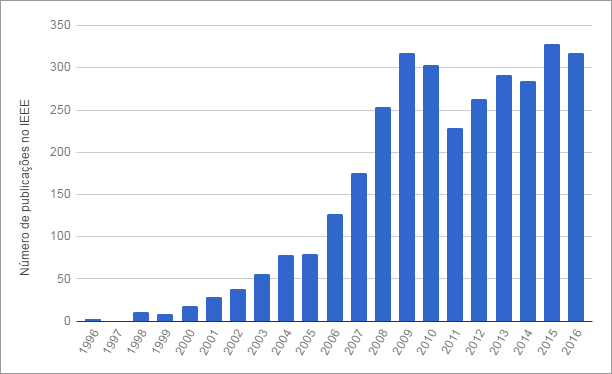
\includegraphics[width=\textwidth]{dados/figuras/steg_graph.png}
	\caption{O crescimento de artigos publicados anualmente pelo IEEE contendo as palavras ``steganography'' ou ``steganalysis'' (Autoria própria).}
	\label{fig:ieee-steganography}
\end{figure}

No contexto deste trabalho, serão consideradas imagens como mídias para comunicação. A maior parte dos métodos de esteganálise em imagens possuem uma formulação que baseia-se em um problema de classificação binária (se tem ou não tem a mensagem escondida). É importante ressaltar que, em contraste com a criptoanálise, não é preciso conseguir ler a mensagem escondida para quebrar o sistema esteganográfico - tarefa de uma área chamada Esteganálise Forense~\cite{fridrich2009steganography}. 

No caso da classificação binária, os métodos são comumente construídos em dois passos: extração de características e classificação. A primeira parte é geralmente feita com algoritmos já bem estabelecidos, incluindo \textit{Subtractive Pixel Adjacency Matrix} (\textit{SPAM})~\cite{spam} e o \textit{Steganalysis Rich Models} (SRM)~\cite{fridrich2012rich}. A classificação pode ser feita utilizando, por exemplo, \textit{Support Vector Machines} (SVM).

O projeto eficiente dos descritores de esteganálise tem uma ligação direta com a acurácia da classificação e consiste em uma tarefa não trivial, exigindo um vasto conhecimento nas áreas de esteganografia e esteganálise. Com o objetivo de contornar esses problemas, soluções baseadas em abordagens de aprendizagem profunda foram propostas~\cite{tan2014stacked,qian2015deep,cnn_base,xu2016ensemble}. Neste contexto, as características utilizadas no processo de classificação são definidas (aprendidas) pela própria rede de aprendizagem~\cite{wu2017deep}.

Este trabalho propõe uma metodologia para comparação de duas diferentes abordagens de esteganálise em imagens digitais: (a) utilizando o descritor denominado \textit{Spatial Rich Models} (SRM) com um conjunto de classificadores do tipo \textit{Fisher Linear Discriminant} e (b) utilizando aprendizagem profunda, do inglês \textit{Deep Learning}, mais especificamente uma rede neural convolucional (do inglês, Convolutional Neural Network - CNN) inspirada naquela implementada por \citeonline{cnn_base}. 

Para criar as bases de treinamento e teste, são considerados três algoritmos de esteganografia espacial adaptativos: \textit{Highly Undetectable Stego} (HUGO)~\cite{hugo}, \textit{Minimizing the Power of Optimal Detector} (MiPOD)~\cite{sedighi2016content} e \textit{Spatial Universal Wavelet Relative Distortion} (S-UNIWARD)~\cite{holub2014universal}. Eles são aplicados nas imagens da base BOSSBase~\cite{bas2011break} utilizando diferentes parâmetros, visando criar cenários para avaliação. 

Para cada cenário criado, foi gerado uma instância do classificador da abordagem (a) e uma instância do classificador da abordagem (b). Todos os classificadores são testados com todos os cenários gerados. Através dessa metodologia que é análoga a criação de múltiplos cenários estegoanalíticos, foi possível avaliar as abordagens de esteganálise estudadas, tanto ao comparar o desempenho da combinação de diferentes algoritmos de esteganografia nas etapas de treinamento e teste quanto ao avaliar o impacto da utilização de diferentes proporções de mensagens escondidas nas imagens (\textit{payloads}).

O uso dos descritores SRM com um conjunto de classificadores apresentou melhores resultados quando se tem informação prévia do algoritmo utilizado, i.e., quando foi utilizado o mesmo cenário para treinamento e teste. Já para a abordagem baseada em aprendizagem profunda os resultados mostraram uma capacidade de generalização maior, dado que a CNN obteve resultados com pouca diferença significativa para diferentes cenários (apenas a diferença de acurácia foi percebida no treinamento para diferentes algoritmos). Esses resultados sugerem que a CNN, por ter maior poder de generalização, pode obter mais sucesso para o uso em esteganálise cega --- onde não há informações sobre o algoritmo de esteganografia utilizado.

Esse trabalho está dividido na seguinte forma: no Capítulo~\ref{chap:revisao_da_literatura} são apresentados conceitos básicos e uma introdução aos métodos de esteganografia, esteganálise e aprendizagem profunda. No Capítulo~\ref{chap:metodologia} estão detalhados a base utilizada, a forma como foram realizados os experimentos e as métricas de comparação. O Capítulo~\ref{chap:resultados} mostra os resultados obtidos com os diversos conjuntos de treinamento. Por fim, são apresentadas as considerações finais e algumas sugestões de trabalhos futuros.


% \section{Objetivos}
% \label{sec:objetivos}

% \subsection{Objetivo geral}
% \label{subsec:objetivo_geral}
% Propor uma abordagem para esteganálise de imagens digitais baseada em algoritmos de aprendizagem profunda.

% \subsection{Objetivos específicos}
% \label{subsec:objectivos_especificos}
% Este trabalho possui como objetivos específicos:

% \begin{itemize}
% \item Realizar um levantamento sobre as principais técnicas clássicas para esteganálise, buscando-se também bibliotecas que as implementem.
% \item Realizar um levantamento sobre algoritmos de aprendizagem profunda com o propósito de esteganálise.
% \item Compilar um benchmark para testes.
% \item Avaliar o desempenho das diferentes técnicas de esteganálise estudadas para diferentes métodos de esteganografia.
% \item Comparar o desempenho obtido na etapa anterior com aquele da técnica proposta neste trabalho, buscando-se identificar novas contribuições que possam ser adicionadas.
% \end{itemize}

\section{Notação}

Será utilizada a anotação da margem com a Figura~\ref{fig:icone-definicao} para localização rápida de definições de termos utilizados no trabalho. Logo após a figura na anotação de margem, estarão os termos definidos no texto. No texto, os termos estarão em negrito.

\begin{figure}[!htb]
	\center
	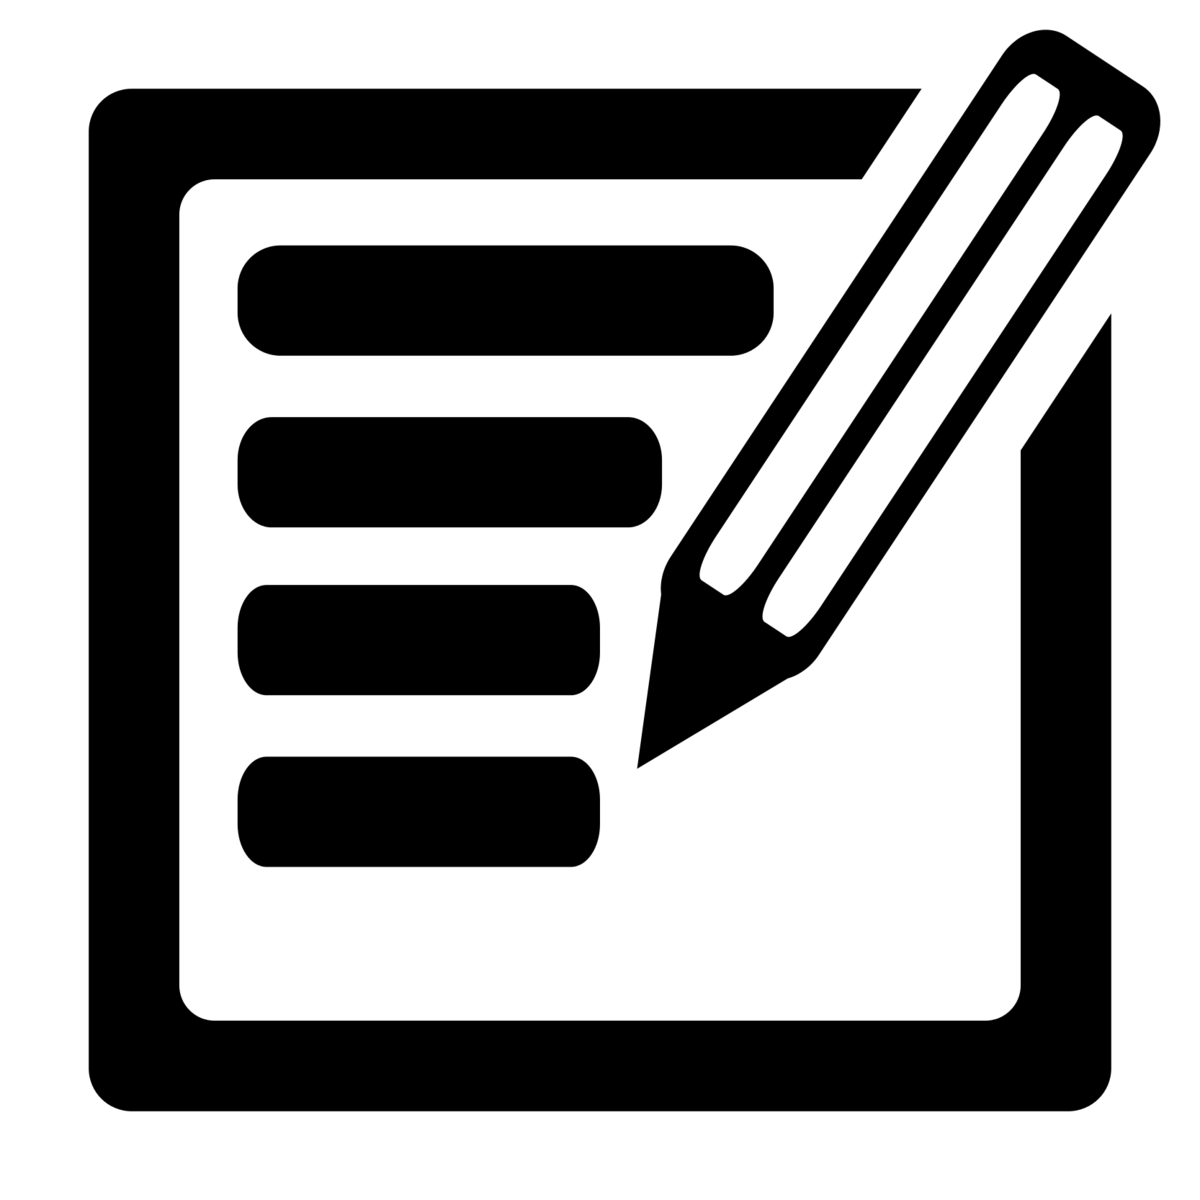
\includegraphics[width=0.1\textwidth]{dados/figuras/icone-definicao.png}
	\caption{Ícone utilizado para a fácil identificação de definições.}
	\label{fig:icone-definicao}
\end{figure}

\definicoes{Exemplo}
Este é um \textbf{exemplo} da utilização da anotação de margem.
